

\documentclass[a4paper]{article}

\usepackage[english]{babel}
\usepackage[utf8]{inputenc}
\usepackage{amsmath}
\usepackage{graphicx}
\usepackage{fancyref}
\usepackage{amsmath}
\usepackage{listings}
\usepackage{url}
\usepackage{float}
\usepackage{amssymb}
\usepackage{rotating}
\usepackage{multirow}
\usepackage[toc,page]{appendix}

\usepackage{tikz}
\usetikzlibrary{shapes}
\usepackage[ruled,linesnumbered,vlined]{algorithm2e}

\usepackage{verbatim}

\newcommand{\norm}[1]{\left\lVert#1\right\rVert}
\newcommand{\argmin}{\arg\!\min}


% taken from manual
\makeatletter
\pgfdeclareshape{document}{
\inheritsavedanchors[from=rectangle] % this is nearly a rectangle
\inheritanchorborder[from=rectangle]
\inheritanchor[from=rectangle]{center}
\inheritanchor[from=rectangle]{north}
\inheritanchor[from=rectangle]{south}
\inheritanchor[from=rectangle]{west}
\inheritanchor[from=rectangle]{east}
% ... and possibly more
\backgroundpath{% this is new
% store lower right in xa/ya and upper right in xb/yb
\southwest \pgf@xa=\pgf@x \pgf@ya=\pgf@y
\northeast \pgf@xb=\pgf@x \pgf@yb=\pgf@y
% compute corner of ‘‘flipped page’’
\pgf@xc=\pgf@xb \advance\pgf@xc by-10pt % this should be a parameter
\pgf@yc=\pgf@yb \advance\pgf@yc by-10pt
% construct main path
\pgfpathmoveto{\pgfpoint{\pgf@xa}{\pgf@ya}}
\pgfpathlineto{\pgfpoint{\pgf@xa}{\pgf@yb}}
\pgfpathlineto{\pgfpoint{\pgf@xc}{\pgf@yb}}
\pgfpathlineto{\pgfpoint{\pgf@xb}{\pgf@yc}}
\pgfpathlineto{\pgfpoint{\pgf@xb}{\pgf@ya}}
\pgfpathclose
% add little corner
\pgfpathmoveto{\pgfpoint{\pgf@xc}{\pgf@yb}}
\pgfpathlineto{\pgfpoint{\pgf@xc}{\pgf@yc}}
\pgfpathlineto{\pgfpoint{\pgf@xb}{\pgf@yc}}
\pgfpathlineto{\pgfpoint{\pgf@xc}{\pgf@yc}}
}
}
\makeatother


\title{Adversarial training on neural networks.}

\author{Marc Moreaux}

\date{\today}

\begin{document}
\maketitle



\section{Introduction} 
\label{sec:introduction}
	
	This machine learning master thesis is about neural-networks (section \ref{sec:neural_networks}). We'll investigate on a technique called adversarial-learning to know if it can help neural-networks in performing better.


	\subsection{Motivation}
		At the very beginning of this thesis, there is me, the writer. I wanted, from the very first day, to work on neural-networks and more specifically on deep-learning. I wanted so, because deep-learning has become in the last decade the most efficient algorithm at classifying images. 
		I was then searching for a topic. I discovered the work made by Ian J. Goodfellow, Jonathon Shlens and Christian Szegedy. In their publication named "Explaining and Harnessing Adversarial Examples"\cite{goodfellow2014explaining} they motivate that adversarial learning could improve the accuracy of some given neural-networks. After contacting one of the authors of this publication, it appeared that it would be a good contribution to validate their observations on other datasets, since most of their test are based on the MNIST dataset\cite{lecun-mnist}. Therefore, the following thesis is about further validating the proposed adversarial-learning method described in \cite{goodfellow2014explaining} with different parameter and different databases.

	\subsection{Methodology}
		We are therefore going to investigate on how is adversarial-learning performing on specific neural-networks called shallow-neural-networks. For the investigation we'll evaluate the impact of some parameters on the network and will also evaluate the model on differnet databases. On the same time, we are going to investigate on the reasons underlining the adversarial performances. To do so, we will first re-implement the proposed solution of \cite{goodfellow2014explaining} in such a way that we isolate adversarial-learning from other techniques used in the paper. At this point we will emphasize the benefits of adversarial-learning. 

		We will then move to another dataset similar to the first one, there will also be 10 different classes of images to classify. That dataset will be the CIFAR10\cite{CIFAR10_BITCHES}. Again, some knowledge will be acquired from this experience. Finally, we will test the adversarial-learning on a dataset of other nature. The one we would try is a phoneme dataset: the TIMIT dataset\cite{maybe...}. The results obtained from this dataset will further validate the technique as useful for classification in the context of shallow-neural-network.

	\subsection{Expected outcome}
		In their paper, Ian J. Goodfellow, Jonathon Shlens and Christian Szegedy, described their technique to able to ??? 
		=> How adversarial learning best separate the classes.
		With this adversarial-learning technique we expect the network to learn the differences between classes more than just the pattern of a class.


	\subsection{Adversarial-learning}
		Until now, we've been speaking a lot of adversarial-learning without explaining what it is about. Lets start off with mentioning what an adversarial sample to a classifier would be. Imagine you have full knowledge of a given classifier. Starting from there, you can create samples to this classifier that are going to give some predictions. Knowing how does the classifier behaves, you can creates samples leading your classifier to some mistakes. This are adversarial samples. In machine learning, adversarial-learning is about creating a classifier resisting to adversarial samples.

		In the publication that interest us\cite{goodfellow2014explaining}, the authors noticed that twisting each pixels of the input images by some very specific values (the adversarial values), an accurate classifier could be easily fooled. Lets detail : Consider you have a classifier able to recognize the MNIST dataset and this classifier makes 10 errors when guessing the classes of 200 samples. Now, if you modify each pixels of these 200 samples by a little value, the classifier makes 180 errors. You've fooled your classifier with adversarial samples.

		The adversarial-learning algorithm we use is going to learn from adversarial samples. Therefore, at any time the algorithm want to predict the class of a sample, he will predict the class of the adversarial sample. It's with this approach that we aim at diminishing the error rate of the classifier.


	\subsection{Running example}
		On the next sections we will explain what are neural-networks, how do we train them and how adversarial-learning apply to them. All along these explanations we will use an example to illustrate our 'propos'.


		The \textbf{task} of our example is to predict the class of an image. There is 3 types of images, a \textit{dot}, a \textit{column} and a \textit{comma}. When a sample is called to be a \textit{dot}, it is referred as belonging to class $y=1$. When it's a \textit{comma}, a class $y=2$ and a \textit{column} a class $y=3$.

		The \textbf{inputs} to our examples are images. They are gray-scaled and have 3 pixels with values in range $[0,1]$. The 3 pixels are aligned in a column such that there is an upper pixel ($x_1$), a middle pixel ($x_2$) and a lower pixel ($x_3$). 

		On the training dataset we have 2 samples for each classes. It is with these examples that we are going to train our classifier.
		$$ \boldsymbol{x}^1 = \left( \begin{matrix} 0  \\ 0  \\ 1  \end{matrix}\right) \text{ ; }
		   \boldsymbol{x}^2 = \left( \begin{matrix} 0  \\ .1 \\ .9 \end{matrix}\right) \text{ ; }
		   y^1 = y^2 = 1 $$

		$$ \boldsymbol{x}^3 = \left( \begin{matrix} 0  \\ 1  \\ 1  \end{matrix}\right) \text{ ; }
		   \boldsymbol{x}^4 = \left( \begin{matrix} .1 \\ .9 \\ .9 \end{matrix}\right) \text{ ; }
		   y^3 = y^4 = 2 $$

		$$ \boldsymbol{x}^5 = \left( \begin{matrix} 1  \\ 0  \\ 1  \end{matrix}\right) \text{ ; }
		   \boldsymbol{x}^6 = \left( \begin{matrix} .9 \\ .1 \\ .9 \end{matrix}\right) \text{ ; }
		   y^5 = y^6 = 3 $$
		Where $\boldsymbol{x}^i$ refer to the input sample $i$ and $y^i$ refer to the class of sample $i$.

		The \textbf{model} we are going to use is a neural-network. Because it has few layers, it's also referred as a shallow-neural-network. Our simple neural-network will have 3 inputs, one for each pixel of the images, 3 hidden neurons and 3 output neurons. \Fref{fig:simple_NN} is a graphical representation of our model.

		\begin{figure}
			\centering
			\def\layersep{2cm}	
			\begin{tikzpicture}[shorten >=1pt,->,draw=black!50, node distance=\layersep]
			    \tikzstyle{every pin edge}=[<-,shorten <=1pt]
			    \tikzstyle{pixel} = [rectangle, fill=black!10,minimum size=17pt,inner sep=0pt]
			    \tikzstyle{neuron}=[circle,fill=black!25,minimum size=17pt,inner sep=0pt]
			    \tikzstyle{annot} = [text width=5em, text centered]
			    \tikzstyle{annot2} = [text width=18em, text centered]
				\tikzstyle{accolade} = [rectangle, text centered, minimum size=17pt]
			    
			    %%% DRAW THE NODES
			    \foreach \name / \y in {1,2,3}
			        \node[pixel] (I-\name) at (0,-\y) {$x^i_\y$};
			    \foreach \name / \y in {1,...,3}
					\node[neuron] (H-\y) at (\layersep*1,-\y) {};
				\foreach \name / \y in {1,...,3}	
					\node[neuron] (O-\y) at (\layersep*2,-\y) {};
				\foreach \name / \y in {1,...,3}
					\node[annot] (P-\y) at (\layersep*3,-\y) {$p^i_\y$};

			    %%% DRAW THE PATHS
			    \foreach \source in {1,...,3}
			        \foreach \dest in {1,...,3}
			            \path (I-\source) edge (H-\dest);

			    \foreach \source in {1,...,3}
			        \foreach \dest in {1,...,3}
			            \path (H-\source) edge (O-\dest);

			    \foreach \source in {1,...,3}
			            \path (O-\source) edge (P-\source);

			    %%% ANOTATE
			    \node[annot,above of=I-1, node distance=1cm] (iv) {Pixels};
			    \node[annot,above of=H-1, node distance=1cm] () {Hidden Neurons};
			    \node[annot,above of=O-1, node distance=1cm] () {Output Neurons};
			    \node[annot,above of=P-1, node distance=1cm] () {Predictions};

			\end{tikzpicture}
			\caption{Simple example of shallow-neural-network}
			\label{fig:simple_NN}
		\end{figure}










	% 	To understand our adversarial training we will use a simple neural network composed by two sigmoid neurons (see section \ref{sec:Artificial_neurons}). The network aims a recognizing a columns and a dot in a three by one pixels image. This network is sketched on \fref{fig:2N_NN}. Considering a white pixel has value $1$ and a dark pixel has value $0$, a column could be represented by a vector $x^1 = [1,0,1]$ and a dot could be by $x^2 = [0,0,1]$. We consider the column to be the output $y^i = 0$ and the dot to be the output $y^i = 1$
	% 	To predict a sensible value, a two-sigmoid network could use the weights and biases :
	% 	$$ W = \left( \begin{matrix} 1 & -1 \\ -1 & -1 \\ 1 & 1 \end{matrix} \right) ; b = \left( \begin{matrix} -1.5 & 0.5 \end{matrix} \right)$$
		
	% 	\vskip 1em
	% 	\textbf{signal propagation: } The input signal $x^i$ propagates through the network resulting in a prediction vector $p^i = \sigma(W^Tx + b)$. To know how right or wrong is this prediction vector, we would use a cost function like the negative log-likelihood:
	% 	$$ C^i = y^i \ln(p^i) + (1-y^i)\ln(1-p^i) $$
	% 	Propagating $x^1$ and $x^2$, we get that $p^1 = [\sigma(.5), \sigma(-.5)]$ and $p^2 = [\sigma(-.5), \sigma(.5)]$

	% 	\begin{figure}
	% 		\centering
	% 		\def\layersep{1.5cm}	
	% 		\begin{tikzpicture}[shorten >=1pt,->,draw=black!50, node distance=\layersep]
	% 		    \tikzstyle{every pin edge}=[<-,shorten <=1pt]
	% 		    \tikzstyle{pixel} = [rectangle, fill=black!10,minimum size=17pt,inner sep=0pt]
	% 		    \tikzstyle{neuron}=[circle,fill=black!25,minimum size=17pt,inner sep=0pt]
	% 		    \tikzstyle{annot} = [text width=5em, text centered]
	% 		    \tikzstyle{annot2} = [text width=18em, text centered]
	% 			\tikzstyle{accolade} = [rectangle, text centered, minimum size=17pt]
			    
	% 		    %%% DRAW THE NODES
	% 		    \foreach \name / \y in {1,2,3}
	% 		        \node[pixel] (I-\name) at (0,-\y) {$x^i_\y$};
	% 		    \node[] (I-4) at (\layersep/2,-3.5) {$1$};
	% 		    \foreach \name / \y in {1,2}
	% 				\node[neuron] (O-\y) at (\layersep*2,-\y-0.5) {$\sigma(z_\y)$};
	% 			\foreach \name / \y in {1,2}	
	% 				\node[] (C-\y) at (\layersep*3,-\y-0.5) {$p^i_\y$};

	% 		    %%% DRAW THE PATHS
	% 		    \foreach \source in {1,...,4}
	% 		        \foreach \dest in {1,2}
	% 		            \path (I-\source) edge (O-\dest);
	% 		    \foreach \y in {1,2}
	% 		        \path (O-\y) edge (C-\y);

	% 		    %%% ANOTATE
	% 		    \node[accolade] at (\layersep*3+1em,-2) { \Huge\} };
	% 		    \node[annot2] at (\layersep*3+10.5em,-2) (cost) {$C^i = \sum_k y^i_k \ln(p^i_k) + (1-y^i_k)\ln(1-p^i_k) $};

	% 		    \node[annot,above of=I-1, node distance=1cm] (iv) {Pixels};
	% 		    \node[annot,above of=O-1, node distance=1cm] (iv) {Neurons};
	% 		    \node[annot,above of=cost, node distance=1cm] (iv) {Cost};

	% 		\end{tikzpicture}
	% 		\label{fig:2N_NN}
	% 		\caption{Two neurons neural network}
	% 	\end{figure}


	% \subsection{Adversarial learning}
	% 	Imagine you are allowed to modify each pixels of our image by a value $\epsilon$. Intuitively, if you want to improve the recognition, you would increase the contrast in the picture and insist on the dots where the aught to be. On the other hand, if you want to confuse the recognition, you would lower the contrast and add color where there shouldn't be.

	% 	These properties are the ones we aught to enforce with our adversarial learning. For an epsilon small enough, we subtract to $x^i$ $\epsilon$ times the sign of the derivative with respect to $x^i$ of the Cost $C^i$.
	% 	$$ x^{i_{\text{adv}}} \leftarrow x^i - \epsilon \text{ sign}(\nabla_{x^i} C^i) $$
	% 	Therefore the input $x^i$ is modified such that ?? TODO: HERE IS THE THING ??

	% 	\vskip 1em
	% 	\textbf{In our example. } We apply the adversarial learning to our example. First we compute the derivative of the Cost with respect to $x^i$. (The mathematics behind this derivative is detailed on the appendix \ref{sec:2N_NN_cost})
	% 	$$	\frac{\delta C^i}{\delta x^i} = W \cdot \left( y^i -p^i \right) $$
	% 	Then we subtract the sign of this derivative to the actual input $x^i$
	% 	\begin{equation}
	% 		\begin{split}
	% 			x^{1_{\text{adv}}} &\leftarrow x^1 - \epsilon \text{ sign}(\nabla_{x^1} C(W,b,x^1)) \\
	% 			x^{1_{\text{adv}}} &\leftarrow x^1 - \epsilon \text{ sign}( W \cdot ( y^i -p^i) )
	% 		\end{split}
	% 	\end{equation}
	% 	\begin{equation}
	% 		x^1 = \left( \begin{matrix} 1 \\ 0 \\ 1 \end{matrix} \right) ;
	% 		x^{1_{\text{adv}}} = \left( \begin{matrix} .7 \\ 0 \\ 1 \end{matrix} \right) ;
	% 		x^2 = \left( \begin{matrix} 0 \\ 0 \\ 1 \end{matrix} \right) ;
	% 		x^{2_{\text{adv}}} = \left( \begin{matrix} .3 \\ 0 \\ 1 \end{matrix} \right) ;
	% 	\end{equation}
		


	% 	Once we have these derivatives, the worst modification we can make to sample $x^i$ is by following this derivative. 
		

	% \subsection{Dataset}
	% 	The first dataset we will be using is the MNIST\ref{??} dataset. This dataset is composed by 60k gray scale images. Each of them represent a hand written digit (6k of each). 


\section{Neural-Networks}
\label{sec:neural_networks}

	In this section we will see how neural-network manage to solve classification tasks. As a reminder, a classification problem aims at identifying the sub-populations of a set belonging to a class. More specifically : if we are given a set of inputs $X$ and outputs $Y$. where $x^i$ denotes a sample from the set $X$ and $y^i$ its class. Then, the aim of classification is to predict the class a new sample given the knowledge based on the $x^i$'s.

	Artificial neural-networks are a family of statistical learning algorithms. They are inspired from the human brain structure : nowadays, we believe the brain has a network of neurons triggering signals over its dendrite and propagated to other neurons through a synapse interface. Network of artificial neurons mimics these properties.

	In this section, we will first introduce what are the artificial neurons and how do we aggregate them to make neural-networks. After we've seen this, we will see how to train these networks: what is a cost and how do we reduce the error made by these networks.


	\subsection{Artificial neuron and Perceptron}
	\label{sec:Artificial_neurons}
		First, the neurons. The first neuron we mention here is the \textbf{Perceptron}. It was described by Rosenblatt in 1958 \cite{rosenblatt1958perceptron} and was one of the first artificial neuron introduced in the literature. This neuron takes as an input multiple binary values to which it apply weights. Once multiplied, these \textit{weighted inputs} are summed-up. If the sum is lower than zero, the neuron outputs zero. Otherwise, the neuron outputs one. A schema of an artificial neuron is given on \Fref{fig:perceptron}.

		Formally: given an input vector $x$ of size $m$ where $x_i$ is the $i$th element of $x$, the Perceptron defines a weight vector $w$ with same shape as the input vector $x$ and a bias term $b$. Then its transfer function is :

		$$ \text{Perceptron}(x) = \begin{cases}1 & \text{if } \sum_{j=0}^m (w_j \times x_j) + b > 0\\0 & \text{otherwise}\end{cases} $$

		In a vector notation this becomes 

		$$ \text{Perceptron}(x) = \begin{cases}1 & \text{if } w^T \cdot x +b > 0\\0 & \text{otherwise}\end{cases} $$

		\begin{figure}
			\centering
			\def\layersep{1.5cm}
			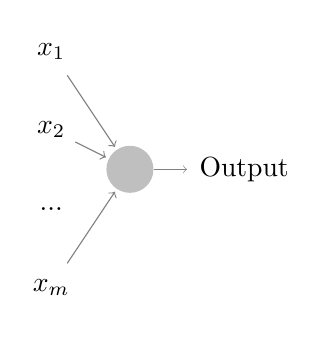
\begin{tikzpicture}[shorten >=1pt,->,draw=black!50, node distance=\layersep]
				\tikzstyle{tata}=[,minimum size=17pt,inner sep=0pt]
			    \tikzstyle{neuron}=[circle,fill=black!25,minimum size=17pt,inner sep=0pt]
			    \tikzstyle{output neuron}=[neuron, fill=red!50];

			    % Input neurons
			    \node[tata] (x1) at (0,-1 cm) {$x_1$};
			    \node[tata] (x2) at (0,-2 cm) {$x_2$};
			    \node[tata] (x3) at (0,-3 cm) {...};
			    \node[tata] (x4) at (0,-4 cm) {$x_m$};
			    
			    % Draw the output layer node
			    \node[neuron,pin={[pin edge={->}]right:Output}] (O) at (\layersep,-2.5) {};

			    % Connect every node in the hidden layer with the output layer
			    \path (x1) edge (O);
			    \path (x2) edge (O);
			    \path (x4) edge (O);

			\end{tikzpicture}
			\label{fig:perceptron}
			\caption{Model of an artificial neuron}
		\end{figure}

		Nowadays we use other types of neurons. As the Perceptron, these neurons consider a weighted sum of their inputs plus a bias term. Now, their activation function is different and their outputs are real valued. We present two of the well known neurons:
		\begin{itemize}
			\item The \textbf{sigmoid neuron} is defined by a smooth threshold function :
			$$ \sigma(x) = \frac{1}{1 + e^{-x}} $$
			\item The \textbf{Regression Logistic Unit} (ReLU) is a neuron which activation function is equal to zero for any negative inputs and equal to its input otherwise.
			$$ \text{ReLU}(x) = \begin{cases} ?? & \text{if } w \cdot x + b > 0 \\0 & \text{otherwise}\end{cases} $$
		\end{itemize}


	\subsection{Neural-network}
		Now that we have neurons, we need a network of them to compose an architecture similar to the brain. The networks we are going to work with are called \textbf{feed-forward} neural-networks. They are the most common ones in the literature. \Fref{fig:feed_forward} is a representation of a two-hidden-layer feed-forward neural-network. As you can see, this model consist of groups of neurons. We denote as layer the group of neurons belonging to the same deepness in the model. Therefore, all the neurons visible on the left in our model, compose the first layer of neurons. It's the input layer. The following layers are called the hidden layers and the last one is the output layer. Some variations exists of this definition, for instance, some outputs of the model might be placed at the same level as some hidden layer.

		Our simple example is also a feed-forward neural-network. It has an input layer fully connected to a hidden layer, which is also fully connected to the output layer. As drawn on the schema with the directions of the arrows, the signal propagates from left to right, from the inputs to the outputs. Because of these two reasons (layers fully connected and single direction signal propagation) our simple example is a feed-forward neural-network.		

		\begin{figure}
			\centering
			\def\layersep{1.5cm}
			\begin{tikzpicture}[shorten >=1pt,->,draw=black!50, node distance=\layersep]
			    \tikzstyle{every pin edge}=[<-,shorten <=1pt]
			    \tikzstyle{neuron}=[circle,fill=black!25,minimum size=17pt,inner sep=0pt]
			    \tikzstyle{annot} = [text width=4em, text centered]


			    %%%%%%%%%%%%%%%%%%%%%%%%%%%%%%%%%%%%%%%%%%%% 
			    %%% DRAW THE NODES
			    %%%%%%%%%%%%%%%%%%%%%%%%%%%%%%%%%%%%%%%%%%%%
			    \foreach \name / \y in {1,...,4}
			        \node[] (I-\name) at (0,-\y) {$x_{i\y}$};

			    \foreach \name / \y in {1,...,5}
			        \path[yshift=0.5cm] node[neuron] (H1-\name) at (\layersep,-\y cm) {};

				\foreach \name / \y in {1,...,7}
			        \path[yshift=1.5cm] node[neuron] (H2-\name) at (\layersep*2,-\y cm) {};   

		       	
			    \node[neuron,pin={[pin edge={->}]right:$p_{i1}$}, right of=H2-3] (O-1) {};
			    \node[neuron,pin={[pin edge={->}]right:$p_{i2}$}, right of=H2-5] (O-2) {};

			    %%%%%%%%%%%%%%%%%%%%%%%%%%%%%%%%%%%%%%%%%%%% 
			    %%% DRAW THE PATHS
			    %%%%%%%%%%%%%%%%%%%%%%%%%%%%%%%%%%%%%%%%%%%%
			    \foreach \source in {1,...,4}
			        \foreach \dest in {1,...,5}
			            \path (I-\source) edge (H1-\dest);

			    \foreach \source in {1,...,5}
			        \foreach \dest in {1,...,7}
			            \path (H1-\source) edge (H2-\dest);

			    \foreach \source in {1,...,7}
			    	\foreach \dest in {1,...,2}
				        \path (H2-\source) edge (O-\dest);

			    % Annotate the layers
			    \node[annot,above of=H2-1, node distance=1cm] (hl) {Hidden layer 2};
			    \node[annot,left of=hl] (hl1) {Hidden layer 1};
			    \node[annot,left of=hl1] {Input layer};
			    \node[annot,right of=hl] {Output layer};
			\end{tikzpicture}
			\label{fig:feed_forward}
			\caption{Feed-forward neural-network with two hidden layers}
		\end{figure}


		It's good to mention that other types of network exits such as the \textbf{recurrent networks}. In these networks, there is directed cycles on the graph which means that a neuron can depends on its own output. This model is considered to be closer to the brain structure but the challenge on training these models isn't state of the art. We won't work on these models.

		\textbf{Symmetrically connected} networks is an other types of network, they are called the "Boltzmann machines". They are symmetrical in the sense that connections between neurons exists in the two directions and the weight on this connections is the same in both directions. Here again, we won't work on these models.


	\subsection{Forward propagation}
		

	

	\subsection{Cost function}
		Once we have build our model, we consider a cost function, also called "loss function". This cost function define how good is the model considering an evaluation criterion. In the case of classification, we want to evaluate how good the prediction is doing towards the true output.
		The most famous cost functions in neural-network classification are the squared error and the cross entropy (also called the "negative log-likelihood"). They are defined as follows for a given sample $i$ and output $j$.
		\begin{itemize}
			\item Squared error : $$ l(p_{ij},y_{ij}) = \norm{y_{ij} - p_{ij}}_2^2 $$
			\item Cross entropy : $$ l(p_{ij},y_{ij}) = -\ln(p_{ij})_{y_{ij}}  ??? $$ 
		\end{itemize}

		Lets take an example. Consider the model presented on \fref{fig:feed_forward}. To this model, we input $x_i$ and propagate the signal until the last layer. This last layer gives us the prediction $p_i = [0.9,0.15]$. Given with $x_i$ we had its true prediction $y_i = [1,0]$. We have everything to compute the two loss functions described earlier : 
		\begin{itemize}
			\item Squared error : $$ l(p_{ij},y_{ij}) =  .1^2 + .15^2 $$
			\item Cross entropy : $$ l(p_{ij},y_{ij}) = -\ln(.1)  $$
		\end{itemize}


	\subsection{Back-propagation}
		Back propagation is the 


		\vspace{1em}
		\textbf{Notation : }\\


	\subsection{Gradient descent}

	\section{Multi-layer neural-network}
		The softmax network we've been previoulsy working with is a single-layer  neural-network, composed by softmax units (or softmax neurons). We are now going to work on a network containing more layers. Instead of forwarding our input data $X$ into the softmax units, we will input them into Rectified Linear Units (ReLU).

		\subsection{Rectifiect Linear Units}
		A ReLU is similar to a perceptron but it has a different transfert function. As the perceptron, it has many inputs an one output. The output is a function of the sum of the weighted inputs. This function is defined as :
		$$ h_t(x) =  $$
		All together, the ReLU outputs :
		$$ \text{ReLU}(X) =  (W^Tx_i) $$

		\subsection{Defining the multi-layer net}
		The Multi-layer neural-network we first study has two layers of composed by 500 ReLU neuron each and an output layer of softmax units. 
% 
\section{Softmax} 
\label{sec:softmax}

	We now study the softmax network. Softmax network is a generalization of logistic regression with a sigmoid transfer function. 
	The softmax network, or better said, the softmax layer, outputs a vector summing to one. 

	Here also we consider $x_i \in \mathbb{R}^m$, the input samples from the set $X$ of size $n$ and $y_i$, the output samples from the set $Y$ of size $n$. The output samples correspond in an integer representing the class of the input. We consider there is $k$ possible classes.

	Considering a softmax layer of size $K$ and with $L$ inputs, the softmax function for a neuron $x$ of the layer is defined as follows :
	$$ \text{softmax}(z_{x}) = \sigma(z_{x}) = \frac{e^{z_{x}}}{\sum_{k\in K} e^{z_k}} $$
	The division by the sum of exponentials permits to have the layer summing up to one. For this reason, we can consider the softmax layer to be a normalized output (throughout the layer) of each of the exponential of the $K$ inputs. 

	On the network visible on \fref{fig:softmax}, the signal propagates as follows : First, the input $x_i$ is multiplied with a weight $w_k$, which result in $z_k$, then $\sigma{z_k}$ is computed. 

	\subsection{Softmax derivatives}
		To be able to apply the gradient descent we compute the derivatives of the softmax. Two cases have to be considered. 
		\begin{itemize}
			\item When we derive $\sigma(z_l)$ with respect to $z_l$.
			\begin{equation} \label{eq:grad_sima_zk1}
				\begin{split}
					\frac{\partial \sigma(z_l)}{\partial z_l} 
					&= \frac{ e^{z_l} \sum_{k} e^{z_k} - e^{z_l} e^{z_l}}{ (\sum_{k} e^{z_k})^2 } \\
					&= \frac{ e^{z_l} \sum_{k} e^{z_k} }{ (\sum_{k} e^{z_k})^2 } - \frac{ (e^{z_l})^2 }{ (\sum_{k} e^{z_k})^2 }\\
					&= \sigma(z_l) - \sigma(z_l)^2 \\
					&= \sigma(z_l)(1-\sigma(z_l))
				\end{split}
			\end{equation}

			\item When we derive $\sigma(z_l)$ with respect to any of the other $z_{k}$ inputs ($k != l$).
			\begin{equation} \label{eq:grad_sima_zk}
				\begin{split}
					\frac{\partial \sigma(z_l)}{\partial z_{k}}
					&= \frac{ - e^{z_l} e^{z_{k}}}{ (\sum_{k} e^{z_k})^2 } \\
					&= - \frac{ e^{z_l} }{ \sum_{k} e^{z_k} } \frac{ e^{z_{k}} }{ \sum_{k} e^{z_k} }\\
					&= - \sigma(z_l)\sigma(z_{k})
				\end{split}
			\end{equation}
		\end{itemize}


	\subsection{Cost function}
		The formulation of the cost function we use with the softmax function depends on the format of the output. The outputs can either be a number representing an index of the true prediction or a binary vector with $K$ values and a single "1" value representing the true prediction.

		Even though the MNIST \footnote{WTF MNIST} dataset is given with an integer valued output representing the index of the output. We will use the binary representation as it shrinks the notation:

		\begin{equation} \label{eq:cost_sigma}
			\begin{split}
				\text{Cost}^i = - \sum_x \left[ y^i_x \log (\hat{y}^i_x) \right]
			\end{split}
		\end{equation}

		Where $\hat{y}_i$ is our prediction (the softmax function) and $1\{k=y_i\}$ is equal to $1$ if the condition in the bracket is true, and $0$ otherwise. This equation \ref{eq:cost_sigma} shows that the cost of sample $i$ only depends on our prediction to be correct. 

	\subsection{Gradient descent}
		To apply the gradient descent algorithm, we compute the derivative of the cost function with respect to the inputs. To improve the readability, we use the term $z_k = w_k^T x$ and $\hat{y}^i_k = \sigma(z^i_{k})$.

		\begin{equation} \label{eq:grad_cost_sigma}
			\begin{split}
				\frac{\partial \text{Cost}}{\partial z_k}
				&= - \sum_x \left[ \frac{y_x}{\hat{y}_x} \frac{\partial \hat{y}_x}{\partial z_k} \right]  \\
				&= \sum_{x!=k} \left[ - \frac{y_x}{\hat{y}_x} \frac{\partial \hat{y}_x}{\partial z_k} \right]  - \frac{y_k}{\hat{y}_{k}} \frac{\partial \hat{y}_k}{\partial z_k} \\
				&= \sum_{x!=k} \left[ - \frac{y_x}{\hat{y}_x} (-\hat{y}_k \hat{y}_x) \right]  - \frac{y_k}{\hat{y}_k} \hat{y}_k (1 - \hat{y}_k) \\
				&= \sum_{x!=k} \left[ y_x \hat{y}_k \right]  - y_k + y_k \hat{y}_k \\
				&= \sum_x \left[ y_x \hat{y}_k \right]  - y_k \\
				&= \hat{y}_k \left[ \sum_k y_x \right]  - y_k \\
				&= \hat{y}_k - y_k
			\end{split}
		\end{equation}

		Putting back the sample index $i$ and deriving the cost with respect to the weights $w_k$:
		\begin{equation} \label{eq:grad_cost_sigma_w}
			\begin{split}
				\frac{\partial \text{Cost}^i}{\partial w_k}
				&= \frac{\partial \text{Cost}^i}{\partial z_k} \frac{\partial z_k}{\partial w_k} \\
				&= (\hat{y}^i_k - y^i_k) x^i_k \\
			\end{split}
		\end{equation}



		\begin{figure}
			\centering
			\def\layersep{2cm}	
			\begin{tikzpicture}[shorten >=1pt,->,draw=black!50, node distance=\layersep]
			    \tikzstyle{every pin edge}=[<-,shorten <=1pt]
			    \tikzstyle{neuron}=[circle,fill=black!25,minimum size=17pt,inner sep=0pt]
			    \tikzstyle{annot} = [text width=6em, text centered]
			    \tikzstyle{annot2} = [text width=1em, text centered]


			    %%%%%%%%%%%%%%%%%%%%%%%%%%%%%%%%%%%%%%%%%%%% 
			    %%% DRAW THE NODES
			    %%%%%%%%%%%%%%%%%%%%%%%%%%%%%%%%%%%%%%%%%%%%
			    \foreach \name / \y in {1,...,5,7}
			        \node[neuron] (I-\name) at (0,-\y) {};
			    \foreach \name / \y in {6}
			    	\node[      ] (I-\name) at (0,-\y) {...};


			    \foreach \name / \y in {1,2}
					\node[] (T-\y) at (\layersep*2,-\y-1) {$z_\y$};
			    \foreach \name / \y in {4}
					\node[] (T-\y) at (\layersep*2,-\y-1) {$z_x$};

				
				\foreach \name / \y in {1,2,4}
					\node[neuron] (O-\y) at (\layersep*3,-\y-1) {};
				
				\node[annot2] at (\layersep*3+1.5em,-2) {$\sigma(z_1)$};
				\node[annot2] at (\layersep*3+1.5em,-3) {$\sigma(z_2)$};
				\node[annot2] at (\layersep*3+1.5em,-5) {$\sigma(z_x)$};

				\node[]       ()    at (\layersep*3,-3-1) {...};
				


			    %%%%%%%%%%%%%%%%%%%%%%%%%%%%%%%%%%%%%%%%%%%% 
			    %%% DRAW THE PATHS
			    %%%%%%%%%%%%%%%%%%%%%%%%%%%%%%%%%%%%%%%%%%%%
			    \foreach \source in {1,...,5,7}
			        \foreach \dest in {1,2,4}
			            \path (I-\source) edge (T-\dest);

			    \foreach \source in {1,2,4}
			        \path (T-\source) edge (O-\source);


			    % Annotate the layers
			    \node[annot,above of=I-1, node distance=1cm] (iv) {Input vector $x^i \in \mathbb{R}^{m_1}$};
			    \node[annot,right of=iv] (void) {};
			    \node[annot,right of=void] (z) {$z_x = w_x^T x^i$};
			    \node[annot,right of=z] {Softmax layer};

			\end{tikzpicture}
			\label{fig:softmax}
			\caption{Feed-forward neural network with two hidden layers}
		\end{figure}



	\subsection{Adversarial learning}
		In section \ref{sec:} we saw the perturbation:
		$$ w^T\tilde{x} = w^Tx + w^T\eta $$
		$$ \eta = \epsilon(\text{sign}(\nabla_x \text{Cost}(w,x,y))) $$

		For the softmax function, the gradient of its cost with respect to the inputs $x^i$ (written below $x$ to simplify the reading) is explained on figure \fref{fig:adversarial_softmax}. As a result, the examples we train are no more $w^T_k x_k$ but their adversarial equivalences $w^T_k \tilde{x}_k$ which depends on the true prediction of the sample.

		When the sample's output is 


		\begin{figure}
			\centering

			\begin{equation}
				\begin{split}
					\text{sign}\left( \frac{\partial \text{Cost}}{\partial x_k} \right)
					&= \text{sign}\left( \frac{\partial \text{Cost}}{\partial z_k} \frac{\partial z_k}{\partial x_k} \right)\\
					&= \text{sign}\left( (\hat{y}_l - y_l) w_k \right)\\
				\end{split}
			\end{equation}

			\begin{tabular}{c||c|c}
				& if $y_l = 0$ & if $y_l = 1$ \\
				\hline
				\hline

				$ \text{sign}\left( (\hat{y}_l - y_l) w_k \right) $ &
				\parbox{12em}{
					\begin{equation}
						\begin{split}
							&  \text{sign}\left( (\hat{y}_l - 0) w_k \right) \\
							&= \text{sign}\left( (\hat{y}_l) w_k \right) \\
							&= \text{sign}\left( (a) w_k \right) * \\
							&= \text{sign}\left( w_k \right) \\
						\end{split}
					\end{equation}
				} & \parbox{12em}{
				\begin{equation}
					\begin{split}
						&  \text{sign}\left( (\hat{y}_l -1) w_k \right) \\
						&= \text{sign}\left( (a-1) w_k \right) *\\
						&= \text{sign}\left( - w_k \right) \\
						&= - \text{sign}\left( w_k \right)
					\end{split}
				\end{equation}
				}\\
				\hline

				$ w^T_k \tilde{x}_k $  &
				\parbox{12em}{
					$$ = w^T_k x + \epsilon w^T_k \text{sign}(w^T_k) $$
					$$ = w^T_k x + \epsilon \norm{w^T_k}_1 $$ }
				&
				\parbox{12em}{
					$$ = w^T_k x - \epsilon w^T_k \text{sign}(w^T_k) $$
					$$ = w^T_k x - \epsilon \norm{w^T_k}_1 $$ }


			\end{tabular} \\ 
			* a is a variable bounded between zero and one : $a\in[0,1]$ \\
			\label{fig:adversarial_softmax}
		\end{figure}


		\begin{table}[h]
		\centering
		%     \begin{adjustbox}{width=\textwidth,center}
		    % \begin{adjustbox}{center}
		        \begin{tabular}{cc||ccccc}

		        	& &  \multicolumn{5}{c}{learning epsilon} \\
		        	& &  $.0$ & $.1$ & $.2$ & $.25$ & $.3$ \\
		            \hline \hline
		            \multirow{8}{*}{adversarial dataset} 
		            	& \multirow{2}{*}{$.0$} & $07,57\%$ & $12,94\%$ & $12,41\%$ & $13,48\%$ & $12,04\%$ \\ 
		            	&                       & $0.2757$  & $0.4640$  & $0.4969$  & $0.5751$  & $0.5246$  \\ \cline{2-7} 
		            	& \multirow{2}{*}{$.1$} & $16,46\%$ & $14,51\%$ & $14,34\%$ & $13,48\%$ & $14,02\%$ \\ 
		            	&                       & $2.6107$  & $0.5485$  & $0.5775$  & $0.5751$  & $0.6300$  \\ \cline{2-7} 
		            	& \multirow{2}{*}{$.2$} & $16,49\%$ & $18,09\%$ & $18,64\%$ & $18,45\%$ & $17,26\%$ \\
		            	&                       & $5.5083$  & $0.8486$  & $0.8872$  & $0.8805$  & $1.0016$  \\ \cline{2-7}
		                & \multirow{2}{*}{$.3$} & $16,50\%$ & $19,99\%$ & $20,61\%$ & $21,28\%$ & $19,00\%$ \\
		                &                       & $8.4112$  & $1.2497$  & $1.3079$  & $1.3155$  & $1.4784$  \\
		            
		        \end{tabular}
		%     \end{adjustbox}
		%     \vspace{ - 05 mm}
		    \caption{xxx}
		    \label{tab:xxx}
		\end{table}



		\begin{table}[h]
		\centering
		%     \begin{adjustbox}{width=\textwidth,center}
		    % \begin{adjustbox}{center}
		        \begin{tabular}{cc||ccccc}

		        	& &  \multicolumn{5}{c}{learning epsilon} \\
		        	& &  $.0$ & $.1$ & $.2$ & $.25$ & $.3$ \\
		            \hline \hline
		            \multirow{8}{*}{adversarial dataset} 
		            	& \multirow{2}{*}{$.0$}  &$0.6562 	$&$0.9352 	$&$1.5566 	$&$1.9000 	$&$2.1495 	$  \\  
		            	&                        &$13.50\%	$&$17.96\%	$&$27.07\%	$&$35.54\%	$&$53.74\%	$  \\ \cline{2-7} 
		            	& \multirow{2}{*}{$.007$}&$0.6816 	$&$0.9565 	$&$1.5645 	$&$1.9027 	$&$2.1502 	$  \\  
		            	&                        &$14.84\%	$&$18.98\%	$&$28.05\%	$&$36.46\%	$&$53.94\%	$  \\ \cline{2-7} 
		            	& \multirow{2}{*}{$.1$}  &$0.6774 	$&$0.9176 	$&$1.5053 	$&$1.8613 	$&$2.1330 	$  \\ 
		            	&                        &$18.93\%	$&$23.71\%	$&$33.81\%	$&$41.97\%	$&$55.87\%	$  \\ \cline{2-7}
		                & \multirow{2}{*}{$.2$}  &$0.8045 	$&$0.9657 	$&$1.4703 	$&$1.8250 	$&$2.1158 	$  \\ 
		                &                        &$24.45\%	$&$30.46\%	$&$41.36\%	$&$48.77\%	$&$59.69\%	$  \\ \cline{2-7}
		                & \multirow{2}{*}{$.25$} &$0.8963 	$&$1.0148 	$&$1.4631 	$&$1.8101 	$&$2.1078 	$  \\ 
		                &                        &$25.68\%	$&$33.32\%	$&$44.66\%	$&$51.60\%	$&$61.66\%	$  \\ \cline{2-7}
		                & \multirow{2}{*}{$.3$}  &$0.9993 	$&$1.0762 	$&$1.4622 	$&$1.7973 	$&$2.1001 	$  \\ 
		                &                        &$26.35\%	$&$35.60\%	$&$47.43\%	$&$54.00\%	$&$63.49\%	$  \\ 

		            
		        \end{tabular}
		%     \end{adjustbox}
		%     \vspace{ - 05 mm}
		    \caption{Softmax}
		    \label{tab:xxx}
		\end{table}

		\begin{table}[h]
		\centering
		%     \begin{adjustbox}{width=\textwidth,center}
		    % \begin{adjustbox}{center}
		        \begin{tabular}{cc||ccccc}

		        	& &  \multicolumn{5}{c}{learning epsilon} \\
		        	& &  $.0$ & $.1$ & $.2$ & $.25$ & $.3$ \\
		            \hline \hline
		            \multirow{8}{*}{adversarial dataset} 
		            	& \multirow{2}{*}{$.0$}  &$0.3137 	$&$1.4646 	$&$1.6651 	$&$1.6474 	$&$1.6700 	$ \\ 
		            	&                        &$8.79\%	$&$30.32\%	$&$34.59\%	$&$34.19\%	$&$36.46\%	$ \\ \cline{2-7} 
		            	& \multirow{2}{*}{$.007$}&$0.3304 	$&$1.5629 	$&$1.6590 	$&$1.6336 	$&$1.6928 	$ \\ 
		            	&                        &$9.74\%	$&$31.92\%	$&$34.87\%	$&$35.54\%	$&$38.38\%	$ \\ \cline{2-7} 
		            	& \multirow{2}{*}{$.1$}  &$1.4000 	$&$1.5643 	$&$1.4565 	$&$1.3650 	$&$1.4427 	$ \\
		            	&                        &$19.03\%	$&$46.34\%	$&$42.87\%	$&$39.81\%	$&$43.08\%	$ \\ \cline{2-7}
		                & \multirow{2}{*}{$.2$}  &$2.5098 	$&$1.6103 	$&$1.3767 	$&$1.2590 	$&$1.3313 	$ \\
		                &                        &$19.57\%	$&$54.92\%	$&$44.98\%	$&$40.76\%	$&$43.49\%	$ \\ \cline{2-7}
		                & \multirow{2}{*}{$.25$} &$2.9940 	$&$1.6362 	$&$1.3653 	$&$1.2483 	$&$1.3191 	$ \\
		                &                        &$19.76\%	$&$57.40\%	$&$45.95\%	$&$41.61\%	$&$44.33\%	$ \\ \cline{2-7}
		                & \multirow{2}{*}{$.3$}  &$3.4552 	$&$1.6628 	$&$1.3660 	$&$1.2548 	$&$1.3264 	$ \\
		                &                        &$19.90\%	$&$59.06\%	$&$46.76\%	$&$42.57\%	$&$45.18\%	$ \\

		            
		        \end{tabular}
		%     \end{adjustbox}
		%     \vspace{ - 05 mm}
		    \caption{Deep net (500-500-10)}
		    \label{tab:xxx}
		\end{table}


		\begin{table}[h]
		\centering
		%     \begin{adjustbox}{width=\textwidth,center}
		    % \begin{adjustbox}{center}
		        \begin{tabular}{cc||ccccc}

		        	& &  \multicolumn{5}{c}{learning epsilon} \\
		        	& &  $.0$ & $.1$ & $.2$ & $.25$ & $.3$ \\
		            \hline \hline
		            \multirow{8}{*}{adversarial dataset} 
		            	& \multirow{2}{*}{$.0$}  &$0.2861 	$&$0.5056 	$&$0.8613 	$& &$0.9940 	$ \\ 
		            	&                        &$8.00\%	$&$11.10\%	$&$14.76\%	$& &$14.99\%	$ \\ \cline{2-7} 
		            	& \multirow{2}{*}{$.007$}&$0.2831 	$&$0.4992 	$&$0.8815 	$& &$0.9821 	$ \\ 
		            	&                        &$8.15\%	$&$11.27\%	$&$14.69\%	$& &$15.06\%	$ \\ \cline{2-7} 
		            	& \multirow{2}{*}{$.1$}  &$0.8532 	$&$0.5810 	$&$0.8736 	$& &$0.9248 	$ \\
		            	&                        &$17.17\%	$&$17.69\%	$&$21.72\%	$& &$21.67\%	$ \\ \cline{2-7}
		                & \multirow{2}{*}{$.2$}  &$1.7098 	$&$0.7990 	$&$0.9509 	$& &$0.9324 	$ \\
		                &                        &$17.62\%	$&$24.30\%	$&$29.19\%	$& &$26.70\%	$ \\ \cline{2-7}
		                & \multirow{2}{*}{$.25$} &$2.0999 	$&$0.9187 	$&$0.9983 	$& &$0.9432 	$ \\
		                &                        &$17.74\%	$&$26.20\%	$&$31.82\%	$& &$28.56\%	$ \\ \cline{2-7}
		                & \multirow{2}{*}{$.3$}  &$2.4700 	$&$1.0381 	$&$1.0473 	$& &$0.9563 	$ \\
		                &                        &$17.88\%	$&$27.29\%	$&$34.26\%	$& &$29.95\%	$ \\
		        \end{tabular}
		%     \end{adjustbox}
		%     \vspace{ - 05 mm}
		    \caption{Deep net (1200-10)}
		    \label{tab:xxx}
		\end{table}



\chapter{Adversarial learning}
\label{sec:adversarial_learning}

	This section is the main contribution of the thesis. We'll see how how an idea of adversarial learning can be applied on a shallow-neural-network. This Idea was first developed by Ian J. Goodfellow, Jonathon Shlens and Christian Szegedy. They proposed an adversarial training on a shallow-feed-forward-neural-network. Along the paper\cite{goodfellow2014explaining}, they emphasize the be benefits of this method applied to a training on the MNIST dataset\cite{lecun-mnist}. Thanks to their adversarial learning, they obtained a better accuracy on the test set.


	
	\section{Intuition}
	\label{sub:intuition}
		With adversarial learning, we train our classifier to resit to samples that could confuse it. On the paper mentioned above\cite{goodfellow2014explaining}, the authors noticed that some adversarial modifications could be made up to fool drastically the classifier. If you were allowed to twist the pixels' values by $.7\%$, and chose carefully these values, you could mislead your classifier from a $95\%$ accuracy to a low $.7\%$. The twist they proposed was adversarial in the sense that they elected a twist given the current classifier. In other words, it's by having full knowledge of the model's neurons and neurons' weights that they created the adversarial twists. These twists are computed with some math and will be detailed on section \ref{sec:creating_the_adversarial_samples}.

		To take advantage of this observation, we will train our model, not on the casual dataset, but on an adversarial version of it. To be more concrete: instead of forward-propagating the input sample through the model and get the prediction out of it, we will twist the input sample and forward-propagate it. The cost will get is the one of the adversarial samples and not of the original dataset.

		With this modification we hope that the classifier will learn, on the one hand, to recognize a class, like it would normally do, but on the other hand, will learn the differences between classes so that it can better discriminate them. 

		

	\section{Creating the adversarial samples}
	\label{sec:creating_the_adversarial_samples}
		The adversarial samples will be created from the original samples. We'll allow ourself to modify the pixels by some values. For instance, for an image, if pixels are coded with values between $0$ and $255$ ($0$ being black and $255$ white) we will allow ourselves to modify the pixels values by $\epsilon_{\text{adv}} \times 255$ so that the image looks the same. The modifications will be based on our feed-forward models weights biases and cost function. Concretely, the adversarial modifications will be equal to:
		$$ \eta = \epsilon_{\text{adv}} \times \text{sign}(\nabla_x \text{Cost}(\boldsymbol{W},\boldsymbol{x},\boldsymbol{y})) $$
		So that the adversarial samples $\boldsymbol{x}$ becomes:
		$$ \tilde{\boldsymbol{x}} = \boldsymbol{x} + \eta $$
		To create an adversarial sample we compute the derivative of the model 


	\section{Adversarial sample on our simple example}
	\label{sub:adversarial_sample_on_the_simple_example}
		Lets now build an example of adversarial sample. As always, we'll use the simple example we've build up (visible on section \ref{sec:weight_initialisation_on_simple_example}) and the sample $\boldsymbol{x}^1$. From those two elements, we'll build-up the adversarial sample corresponding to it.

		We aim at deriving the cost of the model with respect to the inputs $x$. Luckily, we are able to re-use the back-propagation algorithm to compute the derivation. With the notation of section \ref{sec:back_propagation}, we have:
		\begin{equation}
			\begin{split}
				\frac{\nabla_{\boldsymbol{x}} C}{\partial \boldsymbol{x} } 
				&= \frac{\partial \boldsymbol{z}^1}{\partial \boldsymbol{x}} \frac{\partial C}{\partial \boldsymbol{z}^1 } \\
				&= \frac{\partial \left({\boldsymbol{w}^1}^T \boldsymbol{x} + \boldsymbol{b}^1 \right)}{\partial \boldsymbol{x}} \cdot \boldsymbol{\delta}^1 \\
				&= \boldsymbol{W}^1 \cdot \boldsymbol{\delta}^1
			\end{split}
		\end{equation}

		And the modified sample which is the sum of the sample plus a twist $\eta$ is:
		\begin{equation}
			\begin{split}
				\tilde{\boldsymbol{x}}
				&= \boldsymbol{x} + \eta \\
				&= \boldsymbol{x} + \epsilon_{\text{adv}} \times \text{sign}(\nabla_{\boldsymbol{x}} C) \\
				&= \boldsymbol{x} + \epsilon_{\text{adv}} \times \text{sign}( \boldsymbol{W}^1 \cdot \boldsymbol{\delta}^1 )
			\end{split}
			\label{eq:sample_twist}
		\end{equation}

		At this point, we know how to compute the compute an adversarial sample. From the last equation, it doesn't clearly appears that an adversarial sample depends on the variables of the model. Taking a closer look into it, we have that an adversarial sample depends on all the variables present on the model. The neurons' weights appears twice. First on the the back-propagation and then on the forward-propagation (the cost) and the biases appears once on the forward-propagation. We also have that the sample class is present on the cost. Therefore, the adversarial sample needs an entire knowledge on the model and on the samples.

		\vskip 1cm
		Lets apply this to sample $\boldsymbol{x}^1$ with $\epsilon_{\text{adv}} = .07$:
		\begin{equation}
			\begin{split}
				\widetilde{\boldsymbol{x}^1}
				&= \boldsymbol{x}^1 + \epsilon_{\text{adv}} \times \text{sign}( \boldsymbol{W}^1 \cdot \boldsymbol{\delta}^1 ) \\
				&= \boldsymbol{x}^1 + .07 \times \text{sign}
				\left( \left( \begin{matrix}
				-10 	& -10 	& 10 \\
				-10 	& 10 	& -10 \\
				20 		& 10 	& 10 \\
				\end{matrix} \right) \cdot
				\left( \begin{matrix}0 \\ 0.003 \\0.003  \end{matrix} \right) \right)\\
				&= \left( \begin{matrix} 0 \\   0 \\ 1  \end{matrix} \right) +
				\left( \begin{matrix}0.07 \\0.07 \\0.07 \end{matrix} \right) \\
				&= \left( \begin{matrix}0.07 \\0.07 \\1.07 \\\end{matrix} \right)
			\end{split}
		\end{equation}

		From this example we can see the adversarial twist added noise in a direction to confuse the model. This augmented the error made by the model: it went from a loss of $.013501$ to a loss of $.013580$ on the adversarial sample.
		With this example, the benefits of adversarial learning are not clearly visible but we hope that the process underlining adversarial learning is understood.



	\section{MNIST}
	\label{sub:MNIST}
		
		The first dataset we're going to evaluate is the MNIST dataset\cite{lecun-mnist}. This dataset is composed by 70k images representing digits going from 0 to 9. Each of the images has $28*28$ gray scaled pixels. For each pixels is given a value in between 0 and 1 stating how bright is the pixel. The task, given this dataset, is to classify the samples into the 10 classes they belong in. For our needs, we discomposed the dataset into 3 sets: a training-set composed by 50k samples, a validation-set composed by 10k samples and a testing-set composed by 10k samples. 

		From our observations, this dataset is similar to a baseline in machine learning for testing algorithms in image processing. The reason is that it has been around for a long time and that it's big and small enough to quickly and accurately test new ideas related to this domain. It's for this reason that we'll make most of our tests using this dataset.

		Lets now get to adversarial learning. On their paper\cite{goodfellow2014explaining}, the authors used adversarial-learning in conjunction with other techniques. In order separate adversarial-learning from any anther technique, we've decided to re-implement the shallow-neural-network without any method that could be assimilated as a regularization. Concretely, the authors of the paper used two methods that function together called maxout and dropout. Dropout is considered to regularize the network. For this reason we removed it such that our net is only composed by the pixels inputs, the hidden ReLU layer and the softmax output layer. \Fref{fig:mnist_net} is a graphical representation of the MNIST net we used.

		On the following subsections, we are performing some experiments to confirm the benefits of adversarial learning. We'll see the impact of the amount of neurons on the networks, the impact of modifying the adversarial epsilon and compare the adversarial-model with other ones.

		\begin{figure}
			\centering
			\def\layersep{3cm}
			\begin{tikzpicture}[shorten >=1pt,->,draw=black!50, node distance=\layersep]
			    \tikzstyle{every pin edge}=[<-,shorten <=1pt]
			    \tikzstyle{neuron}=[circle,fill=black!25,minimum size=17pt,inner sep=0pt]
			    \tikzstyle{annot} = [text width=4em, text centered]
			    \tikzstyle{pixel} = [rectangle, fill=black!10,minimum size=17pt,inner sep=0pt]


			    %%%%%%%%%%%%%%%%%%%%%%%%%%%%%%%%%%%%%%%%%%%% 
			    %%% DRAW THE NODES
			    %%%%%%%%%%%%%%%%%%%%%%%%%%%%%%%%%%%%%%%%%%%%
			    \foreach \name / \y in {1,...,3}
			        \node[pixel] (I-\name) at (0,-1.5-\y) {$x_{\y}$};
		        \node[]      (I-4) at (0,-1.5-4) {...};
	            \node[pixel] (I-5) at (0,-1.5-5) {$x_{784}$};


			    \foreach \name / \y in {1,...,6}
			    	\node [neuron] (H1-\name) at (\layersep,-\y cm) {};
		    	\node []       (H1-7) at (\layersep,-7 cm) {...};
		    	\node [neuron] (H1-8) at (\layersep,-8 cm) {};

		       	
			    \node[neuron,pin={[pin edge={->}]right:$p_{1}$}, right of=H1-3] (O-1) {};
			    \node[neuron,pin={[pin edge={->}]right:$p_{2}$}, right of=H1-4] (O-2) {};
			    \node[right of=H1-5] (O-3) {...};
			    \node[neuron,pin={[pin edge={->}]right:$p_{10}$}, right of=H1-6] (O-4) {};

			    %%%%%%%%%%%%%%%%%%%%%%%%%%%%%%%%%%%%%%%%%%%% 
			    %%% DRAW THE PATHS
			    %%%%%%%%%%%%%%%%%%%%%%%%%%%%%%%%%%%%%%%%%%%%
			    \foreach \source in {1,...,3,5}
			        \foreach \dest in {1,...,6,8}
			            \path (I-\source) edge (H1-\dest);

			    \foreach \source in {1,...,6,8}
			    	\foreach \dest in {1,...,2,4}
				        \path (H1-\source) edge (O-\dest);

			    % Annotate the layers
			    \node[annot,above of=H1-1, node distance=1cm] (hl1) {Hidden layer};
			    \node[annot,left of=hl1] {Input layer};
			    \node[annot,right of=hl1] {Output layer};
			\end{tikzpicture}
			\caption{Graphical model of a MNIST net}
			\label{fig:mnist_net}
		\end{figure}

		\subsection{Playing with neuron quantities}
		\label{ssub:playing_with_neuron_quantities}
			One of the first experiment we got interested in knowing which parameters should be used to train the neural network. We would expect that the size of the hidden layer has a direct impact on the predictions and on the accuracy of the model. We would therefore try different layer sizes and see which ones were over and under fitting. We also want to know if one of the adversarial or usual training would under or over-fit before the other given the same amount of neurons. If one were to under-fit longer than the other, it would imply it need to learn more functions than the other model to be accurate.

			In other words, if both of the models stops under-fitting on the same time, it would probably mean that both of the models learn the same amounts of functions, but one would be more accurate than the other. On the other hand, if a model (A) under-fits longer than the other model (B) it would probably mean that it (A) needs to learn more functions to accurate than the other model (B).

			For this reason, the we've trained MNIST on models with different amount of weights. Each of the adversarial examples are trained with $\epsilon_{\text{adv}} = .25$. The graph on \fref{fig:mnist_neurons} shows the evolution of the accuracy and the confidence for the adversarial and non-adversarial models while increasing the amount of neurons. As one could expect, the accuracy is defined as :
			$$\text{acc} = \frac{\text{\#correct guesses}}{\text{\#samples}}$$ 
			And the confidence reflects how much the model was sure of which ever predictions it made 
			$$\text{conf} =  \text{mean}( \text{argmax} (\text{predictions}))$$

			\begin{figure}
				\centering
				\includegraphics[width=0.7\textwidth]{/home/marc/git/MI10_adversarial_training/training_test/MLP3/mem/bar_neuron_impact.png}
				\caption{Comparing the amount of neurons' impact on non-adversarial and adversarial models. Every pair represent a non-adversarial-learning and an adversarial-learning trained with a certain amount of hidden neurons.}
				\label{fig:mnist_neurons}
			\end{figure}

			\vskip 1cm
			\textbf{Analysis:}\\
			Looking at this graph (\fref{fig:mnist_neurons}), the first thing we notice is that adversarial-learning performs worse than non-adversarial-learning for models with less than a hundred neurons. When we deal with 5 hidden neurons, adversarial model is 17 percent points less accurate than the non-adversarial model. With this observation we can hypothesize that adversarial model can't properly synthesize what it sees with so few functions (neurons). Therefore it introduces more inaccuracy in the functions it learns.

			What we find more relevant is the following: the adversarial-learning plateaus at 400 neurons whereas non-adversarial-learning plateau in between 50 and 100 neurons. In other words, adversarial-learning need far more neurons (far more functions) to reach its best accuracy. From this observation, and from the insight of the universal approximator \cite{hornik1989multilayer}, we can say that adversarial-learning learns more functions than the other model does. Which is to say that the adversarial-learning method is not about having the same kind of model but one being more accurate than the other. It's about having a new model learning far more  functions. Also, as the adversarial-learning models converges slower than the other model, I would say that adversarial-learning learns a whole set of new functions. If it were not the case, We would expect the adversarial models to be at least as good as the non-adversarial.



		\subsection{Playing with adversarial epsilon}
		\label{ssub:playing_with_adversarial_epsilon}
			The Adversarial learning we use relies on an epsilon, the one we've noted $\epsilon_{\text{adv}}$:
			$$ \boldsymbol{x} + \epsilon_{\text{adv}} \times \text{sign}(\nabla_{\boldsymbol{x}} C) $$
			In this subsection, we want to evaluate the impact of this value on the learning. We are going to expose the learning of a 800 hidden-neurons net trained with different $\epsilon_{\text{adv}}$. Even though, we expect an increased accuracy with an increased epsilon, we don't have any idea on which epsilon would be better. 

			\begin{figure}
				\centering
				\includegraphics[width=0.7\textwidth]{/home/marc/git/MI10_adversarial_training/training_test/MLP3/mem/bar_eps_imapct.png}
				\caption{Evaluate non-adversarial and adversarial models of 800 hidden neurons.}
				\label{fig:mnist_adv_eps}
			\end{figure}
			
			\vskip 1cm
			\textbf{Analysis:}\\
			\Fref{fig:mnist_adv_eps} seems to reveal that a good adversarial epsilon for this dataset and given a model of 800 neurons is located between $.05$ and $.3$. On the figure we plotted, the optimum value for the adversarial epsilon seems to be $.1$. On this same plot, we can see that the confidence for the predictions falls down as the adversarial epsilon raises. We don't know what these two informations teaches us towards adversarial-learning but that low epsilon value seems to perform better on both accuracy and confidence.


		\subsection{Compare to noisy dataset} 
		\label{ssub:compare_to_noisy_dataset}
			One of the objective mentioned for adversarial-learning was to diminish the linearity of the network: The authors of \cite{goodfellow2014explaining} said that usual networks were not able to understand the underlining nature of a class because it was too much dependent on the underlining distribution of the data present on the dataset. This dependency was described with too much linearity on the network to learn the underlining dataset. It's because of this over-linearity that adversarial samples were so good at fooling the models.

			On this subsection, we want to see if, effectively, the model is better at generalizing. To do this, we are going to compare a non-adversarial model (A) with an adversarial model (B) on modified test-sets. The first one will compare A and B on the adversarial test-set and will most probably confirm the hypothesis seen above.The second one is going to compare A and B on an other modified version of the test-set. Here we'll by twisting each pixels by a random value. This random value comes from a standard normal distribution (with a mean of 0 and variance of 1). To produce this set we compute :
			$$ \tilde{\boldsymbol{x}}^i = \boldsymbol{x}^i + \epsilon_{\text{ads}} \text{noise} $$
			Where noise is randomly generated following a standard normal distribution.
			
			\begin{figure}
				\centering
				\includegraphics[width=0.4\textwidth]{/home/marc/git/MI10_adversarial_training/training_test/MLP3/mem/bar_testset_impact_adv.png}
				\includegraphics[width=0.4\textwidth]{/home/marc/git/MI10_adversarial_training/training_test/MLP3/mem/bar_testset_impact_norm.png}
				\caption{Evaluate non-adversarial (dashed line) and adversarial models (plain line) of 800 hidden neurons on modified test-sets. On the left, we try the two models on an adversarial test-dataset. The horizontal axis represents the epsilon values used to modified the test-set. On the right, we try the two models on an normal-distribution-modified test-dataset with different standard deviations.}
				\label{fig:mnist_adv_noisy_ds}
			\end{figure}
			\begin{figure}
				\centering
				\includegraphics[width=0.7\textwidth]{/home/marc/git/MI10_adversarial_training/training_test/MLP3/mem/bar_noisy_ts_adv.png}
				\includegraphics[width=0.7\textwidth]{/home/marc/git/MI10_adversarial_training/training_test/MLP3/mem/bar_noisy_ts_norm.png}
				\caption{Extract of the test-set with the same image with different noises. On the top, you see the adversarial noised sample with $\epsilon_{\text{ads}} = [.0, .1, .2, .3]$. On the bottom you see the uniform noised sample with, from left to right the standard deviation taking values: $\epsilon_{\text{noise}} = [.0, .1, .2, .3]$}
				\label{fig:mnist_adv_noisy_ds_img}
			\end{figure}

			\vskip 1cm
			\textbf{Analysis:}\\
			With the left plot of \fref{fig:mnist_adv_noisy_ds}, we confirm that adversarial samples easily fools a usual feed-forward model. Twisting the pixels by $10\%$ in the direction of the worst case (our adversarial case),drastically confuses the original model. Now, trying to fool the adversarial-model with this same technique doesn't work as good. The adversarial-model can't be fooled as easily. 

			With the plot on the right, we compare the accuracy of both the models on another twisted dataset. This time, the adversarial-model keeps an advantage until the dataset becomes too noisy $\epsilon_{\text{noise}}=.22$. This result is a bit contradictory with our expectations. In fact, we would have expected that adding noise to this test-set would have fooled more the non-adversarial model than the adversarial one. The reason being that adversarial-learning was supposed to better generalize the underlining distribution of the test-set and therefore be less dependent on noise.

			Despite this, the adversarial-model still outperforms the other one on this modified test-set before the test-set gets really noisy ($\epsilon_{\text{noise}}>.22$ )



		\subsection{Train with noisy dataset}
		\label{ssub:train_with_noisy_dataset}
			So far we've been comparing an usual model to the non-adversarial model. Here, we introduce a new model originating from the previous experience. As a matter of fact, we stated that model A (the usual model) was too much linear. We introduced model B (adversarial-model) as being less dependent on the underlining distribution. Then we tested the models on a noisy test-sets. Now we want to compare B with a new model that is also less dependent on the underlining distribution. Therefore we introduce a model C (also having 800 hidden neurons) that is trained on noisy dataset. This dataset is also computed live. At every iterations of the back-propagation a new test-set is generated (as for the adversarial-model (B)). This live modification of the test set permits the classifier not to over-fit an original noise given to the network. It must learn that noise can appear. The input sample modification is the same a before: 
			$$ \tilde{\boldsymbol{x}}^i = \boldsymbol{x}^i + \epsilon_{\text{ads}} \text{noise} $$
			Where noise is randomly generated following a standard normal distribution.

			As a recall, adversarial-learning modified the input samples towards a worst case prediction given the model. Now, instead of modifying the input sample towards this worst case sample, we twist the sample by adding a random noise. At this point, we don't necessary expect this learning to be better at classifying but we hope that it can better resist to adversarial samples. If it does, it could support that usual training is too much linear.

			\begin{figure}
				\centering
				\includegraphics[width=0.4\textwidth]{/home/marc/git/MI10_adversarial_training/training_test/MLP3/mem/bar_testset_impact_2_adv.png}
				\includegraphics[width=0.4\textwidth]{/home/marc/git/MI10_adversarial_training/training_test/MLP3/mem/bar_testset_impact_2_norm.png}
				\caption{Evaluate normal-distribution-based model versus the casual and adversarial models of 800 hidden neurons on noisy test-sets and adversarial datasets.}
				\label{fig:mnist_noisy_learn}
			\end{figure}

			\vskip 1cm
			\textbf{Analysis:}\\
			With the left plot of \fref{fig:mnist_noisy_learn} we can make two observations. The first one was unexpected and is that model C (new one) performs as good as model B (adversarial model) on the original dataset. They both score close to $98.7\%$ accuracy on the original test-set. The second observation, more interesting to us, reveals that model C is more resistant to adversarial samples than model A. This observation come in favor of A being too linear and relying too much on the original distribution of the samples. Why so ? The objective in training the dataset with model C, was to enforce the classifier to learn that each of the pixels of a class followed a normal distribution. We enforce the model to consider an alternative data distribution than the one present on the original training-set. If C would have performed as bad as A on the adversarial test-set, it could have meant that model A, actually, generalizes and is not as linear as we ought to say.
			With the plot on the right, we have that model C outperforms models A and B. This observation is legitimate with the experiment we've build up. We trained model C on believing that the pixels were under a normal distribution and then tested the model on a test-set enforcing this normal distribution modification. Once again, we are a bit disappointed here that adversarial-learning can't best predict this noisy dataset.

			
		\subsection{Visualizing weights}
		\label{ssub:visualizing_weights}
			We thought it could be nice to visualize what had been learned by the network. We've therefore tried to visualize the weights to find out the patterns it relies on. The \textbf{first} idea that came to our mind was to "back-propagate" the output-neurons' weights connected to the inputs. As a result, we would have visualized a pattern of what was understood as a 1, a 2 or any class of the task. Mathematically we just needed to compute:
			$$ W_{\text{visualize}} = \boldsymbol{W^1} \cdot \boldsymbol{W}^2 $$
			And each of the columns of $W_{\text{visualize}}$ would have represented the patterns learned from a class. On \fref{fig:mnist_weight_class}, you see these weights for classes 0 to 4 of MNIST. The upper-row are casual-learning and the lower-row is adversarial-learning. On both neither of these images we can distinguish the patterns of a one, a two or any other digit.
			\begin{figure}
				\centering
				\includegraphics[width=0.4\textwidth]{/home/marc/git/MI10_adversarial_training/training_test/MLP3/mem/bar_weight_class_800.png}
				\includegraphics[width=0.4\textwidth]{/home/marc/git/MI10_adversarial_training/training_test/MLP3/mem/bar_weight_class_2000.png}
				\caption{Attempt at visualizing classes pattern on casual-model (top) and adversarial-model (bottom) of 800 neurons (left) and 2000 neurons (right).}
				\label{fig:mnist_weight_class}
			\end{figure}
			\begin{figure}
				\centering
				\includegraphics[width=0.3\textwidth]{/home/marc/git/MI10_adversarial_training/training_test/MLP3/mem/bar_weight2_100.png}
				\includegraphics[width=0.3\textwidth]{/home/marc/git/MI10_adversarial_training/training_test/MLP3/mem/bar_weight2_800.png}
				\includegraphics[width=0.3\textwidth]{/home/marc/git/MI10_adversarial_training/training_test/MLP3/mem/bar_weight2_2000.png}
				\caption{Attempt at visualizing neuron patterns on casual-model (top) and adversarial-model (bottom) of 100 neurons (left), 800 neurons (center) and 2000 neurons (right).}
				\label{fig:mnist_weight}
			\end{figure}

			The \textbf{second} way we tried to visualize the patterns was at the first (and only) hidden-layer we have. We've plotted some of the neuron's weight but none gave gave us more insight on what was seeing model A and model B. After watching \fref{fig:mnist_weight}, the only comparison we could make was that the adversarial-model seems to have more grain on its neurons compared to the casual-model.

			After these two failures in visualizing the patterns we expected to have, we've browsed the find and found that this types of networks were not supposed to contain some neurons with the patterns we were looking for. Instead, another model called Restricted Boltzmann Machines (RBM) would have these properties (where you can see patterns learned by neurons).

		\subsection{MNIST summary}
		\label{ssub:mnist_summary}
			With the MNIST dataset we've seen many things. 
			\begin{itemize}
				\item Playing with the hidden neurons quantities we've seen that adversarial-model (B) learned more functions than the usual-model (A) did.
				\item Playing with the adversarial epsilon we've seen which epsilons seemed to perform better.
				\item Comparing models A and B with noisy datasets confirmed that A was sensible to adversarial samples when B was not.
				\item Training a new model (C) on a noisy dataset probably confirmed that A was too linear.
				\item Visualizing weights didn't worked as expected but played a role in knowing what future work could be made of.
			\end{itemize}
		
	
	\section{CIFAR-10}
	\label{sub:cifar_10}
		Another dataset we've used is the CIFAR-10 database. CIFAR-10 is a dataset composed by 60k images. An image is about one of the following 10 classes: \textit{an airplane, an automobile, a bird, a cat, a deer, a dog, a frog, a horse, a ship or a truck}. Each images is composed by $32*32$ RGB pixels which makes an input vector composed by $3072$ values. As for the MNIST dataset, we discomposed the dataset into 3 sets: a training-set composed by 40k samples, a validation-set composed by 10k samples and a testing-set composed by 10k samples. \Fref{fig:cifar} is an extract of the dataset.

		\begin{figure}
			\centering
			\includegraphics[width=0.8\textwidth]{/home/marc/git/MI10_adversarial_training/training_test/MLP3/mem/bar_orig_CIFAR.png}
			\caption{Extract of Cifar10 dataset.}
			\label{fig:cifar}
		\end{figure}


		Right below, we are going to see how adversarial-learning did with CIFAR-10.


		\subsection{Training CIFAR-10} % (fold)
		\label{ssub:training_cifar_10}
			We've build a model to learn CIFAR-10. At the beginning, we trained a model with 3072 inputs, 2500 hidden neurons and 10 outputs. Training this dataset took a huge amount of time (we didn't reached the end). Therefore, we decided to shrink the input vector. To do so, we gray-scaled the input sample. In other words, we changed the RGB pixel to gray pixels. This modification shrank our input by 3 times less inputs values (1024 instead of 3072). Even shrinking the input vector, learning the dataset took 3 days on our computer. Because of this reason, we were not able to perform all the test we performed on MNIST.

			As we did for MNIST, we are going to compare basic model (Ac) and adversarial-model (Bc) to noisy datasets. As before, we'll have an adversarial dataset and a dataset with random noise. Before rnedering the graph, we expect to have the same kind of results. We expect the adversarial samples to fool Ac but not Bc. We expect Bc to be more accurate that Ac is and, maybe we'll have this time Bc performing better than Ac on the random noise test-set. \Fref{fig:cifar_noisy_test} are the resulting plots applied for CIFAR-10.

			\begin{figure}
				\centering
				\includegraphics[width=0.4\textwidth]{/home/marc/git/MI10_adversarial_training/training_test/MLP3/mem/bar_testset_impact_adv_CIFAR.png}
				\includegraphics[width=0.4\textwidth]{/home/marc/git/MI10_adversarial_training/training_test/MLP3/mem/bar_testset_impact_norm_CIFAR.png}
				\caption{Evaluate non-adversarial (dashed line) and adversarial models (plain line) of 2500 hidden neurons on modified test-sets. On the left, we try the two models on an adversarial test-dataset. The horizontal axis represents the epsilon values used to modified the test-set. On the right, we try the two models on an normal-distribution-modified test-dataset with different standard deviations.}
				\label{fig:cifar_noisy_test}
			\end{figure}

			\vskip 1cm
			\textbf{Analysis:}\\
			Looking at the results, we have that Bc outperforms Ac on the original test-set. This observation comes in favor of adversarial-learning being less linear that Ac is. This result is very similar to the one we had with MNIST on section \ref{ssub:compare_to_noisy_dataset}. As before, we see that Ac is easily fooled by adversarial learning and that Bc is not. It appear weird that Bc does an amazing job at classifying the adversarial-test-set, but remember that the noise given to the adversarial-test-set depends on the output. Therefore, building this adversarial-test-set, we gave informations about which classes the samples belonged in.
			As before, also, we have that Bc is not doing an amazing job on the noisy test-set. The adversarial-classifier can't predict a sample with random noise much better than Ac does.

		\subsection{CIFAR summary}
			With this new dataset, we confirm some of the observations we've made earlier with the MNIST dataset. Sadly, the higher dimensionality needed on the models made us unable to recompute all the tests performed earlier.
	

	\section{Covertype dataset}
	\label{sub:covertype_dataset}
		This is the third and last dataset we performed experiments on. This one is called the covertype dataset\footnote{\url{https://archive.ics.uci.edu/ml/datasets/Covertype}}. We elected this dataset because its nature was far from the two image dataset seen previously and because it consists on a multi-class classification task. With this dataset we "classify the predominant kind of tree cover from strictly cartographic variables". The samples belongs in 7 classes and the input vectors are composed by 54 values. Here the 54 values are not necessarily in a given range. It might happen that a value is a numeric encoding.

		\subsection{Training Covertype}
			Learning this dataset was not as successful as learning the two other datasets. We've trained many models hopping to see an adversarial one better than its non-adversarial equivalence but it never really happened. the results we got are the followings:

			\begin{table}[ht]
				\centering
				\begin{tabular}{c||c|c|c|c|c}
					hidden neurons & 60 & 80 & 100 & 120 & 150 \\
					\hline
					non-adversarial & $.5103$ & $.5107$ & $.5116$ & $.5108$ & $.5108$ \\
					adversarial     & $.5106$ & $.5111$ & $.5103$ & $.5106$ & $.5116$ \\
				\end{tabular}
				\caption{Accuracy of adversarial and non-adversarial models with different amount of hidden neurons on the Covertype dataset.}
				\label{tab:cov_acc}
			\end{table}

		\subsection{Covertype summary}
			From this experiment we learn that adversarial-learning won't necessarily perform better non-adversarial-learning on every dataset. The fact that adversarial-learning doesn't perform better here is relevant with the nature of the dataset.


		% # => 150 -> yes
		% 0.511660728731
		% 0.510628044268
		% # => 120 -> no
		% 0.510774341233
		% 0.511152992203
		% # => 100 -> yes
		% 0.510800158345
		% 0.510301027521
		% # => 80 -> yes
		% 0.510757129826
		% 0.510671072787
		% # => 60 -> no
		% 0.510352661744
		% 0.511677940139

	\section{Adversarial learning conclusion}
	\label{sub:adversarial_learning_conclusion}
		Here ends our experiments on the different datasets. we'll come back on the results obtained here in the conclusion. We are now going to see how we implemented these experiments.

\section{Implementation}

	In this section we present the software we chose to implement our solution. The elected software comes from the Lisa-lab\footnote{url{https://github.com/lisa-lab}} in Montreal and is called Pylearn2. The Lisa lab is specialized in neural-network and more specifically, deep learning. Yan Goodfellow, one of the writers of the paper\cite{goodfellow2014explaining}, was part of this institution, he is one of the main contributor of Pylearn2 and write most of his paper with this tool. His implementation of Adversarial-learning was made with this tool. In the following section, we are going to present the software's needs we had with respect to this thesis and on the next one we'll explore the way Pylearn2 works.

	\subsection{software needs}
		At the very beginning of this thesis we searched for a good software with respect to many needs.
		Of course, as we are doing neural-nets, our first need was to have a software able to implement a neural-network. Then there was some other needs. The learning curve for this software had to be steep enough so that we could implement our solution in some reasonable time. After this, the software had to flexible towards our needs of adversarial-learning. Indeed, the cost of our shallow-feed-forward network had to be modified in order to accept adversarial-learning. Also, as we have large databases like the Cifar-10 (composed by $60k$ sample of $3k$ values each), the software's algorithms had to perform fast operations. To show the importance of this criterion, with the software we finally choose, it took us more that 36 hours to compute the adversarial model of Cifar-10.

		In neural networks there was 4 main softwares answering partially our needs.
		\begin{itemize}
			\item Torch: "Torch is a scientific computing framework with wide support for machine learning algorithms". Their framework is very easy to use. In one hour you can build a neural-network classifying MNIST. Now, the implementation of new functions is complicated. Implementing a new cost function is hard, it's for this reason that we didn't chose this soft.
			\item Lush: "Lush is an programming language designed for researchers, experimenters, and engineers interested in large-scale numerical and graphic applications". Even though the description seems appealing, the software isn't maintained and doesn't embed modern gradient descent algorithms. 
			\item Pylearn2: "Pylearn2 is a machine learning library". It was designed for deep-learning, is written in python and can differentiate function. Because it also fulfills all the software needs, this alternative was chosen.
			\item Matlab: The very famous Matlab could have been used for our project. Now the libraries provided weren't as specific as the other softwares.
			\item R: "R is a language and environment for statistical computing and graphics". This language integrates deep-learning algorithms but was not mentioned as a reference in the deep leaning domain.
		\end{itemize}


		Advantage and drawbacks of Pylearn2:

		On the one hand, Pylearn2 is written in Python: a very common and easy to understand language. That makes a big advantage to Pylearn2 toward a soft written in C or Lua. On the other hand, Pylearn2 uses a file format called "Yaml" to build and train the networks. These files are made so that you can easily call classes with many parameters. Though it's practical, it's hard to understand this approach if you've never seen something similar before.
		Pylearn2 is being under development which makes it a software up to date. Now, this advantage is also a drawback as the python documentation isn't as furnished as one could expect nor are the error messages. It was often needed during the implementation to browse specific forums and investigate on which could be a good solution for us. Thought the python documentation lacks of details, a blog is maintained by the Lisa-lab to introduce to their tools.
		At this point, Pylearn2 is far from being the easiest tool to use in order to build and trained a neural-network, but what really came in the balance to support it use is a useful library on which it relies: Theano. Theano, also developed in the Lisa lab. It's "a Python library that allows you to define, optimize, and evaluate mathematical expressions involving multi-dimensional arrays efficiently". This library also include automatic differentiation, so that you can create a new cost function without having to differentiate it by hand.

		I'll finish these motivations mentioning that Pylearn2 is hard to get into. One need to spend some time on the code, on the blog and on the forums to builds its own models but, at the end, Pylearn2 is very flexible and offer a useful tool of differentiation to rapidly test new cost functions.


	\subsection{Pylearn2}
		Lets now present the tool. Pylearn2 is a python library. It mainly relies on Numpy, for matrix manipulation and on Theano, for optimized operations on matrices. There is three main files on Pylearn2: the model, the cost and the routine files. Following comes the description of them. You may watch before \fref{fig:pylearn2} for a graphical representation of the system.
		\begin{itemize}
		  	\item The model: The model is represented by a class in Pylearn2. It has to follow rhe sucture of an abstract class (\textit{pylearn2.models.model.Model}) in order to work with the system. In supervised learning (what we are doing), this model will be called by the cost to compute it. The model, in our case, is a shallow-feed-forward-neural-network. An flexible implementation of this model is already available on the Pylearn2 library.
		  	\item The cost: In Pylearn2 philosophy, one should be able to modify easily the cost to test it. This is the strength of Pylearn2, where you would give the cost and the library will differentiate it. This ease implies some difficulties as the user has to input a cost in a 'Theano-symbolic' format. In the system, this cost is also represented by an abstract class (\textit{pylearn2.costs.cost.Cost}) where the user must implement the 'expr' function which outputs the 'Theano-symbolic' function.
		  	\item The routine: Finally, when one desire to build a model with a specific cost and a specific learning algorithm, one will create a 'yaml' file. This file is only composed by classes calls. For the training, the library expects first the \textit{Train} class containing both the \textit{Model} one and the \textit{Learning algorithm} class which itself contains the \textit{Cost} class. With these classes and the dataset given as parameters of them, Pylearn2 will initiate a learning process.
	  	\end{itemize}
			 
		\begin{figure}[H]
			\centering
			\def\layersep{8em}	
			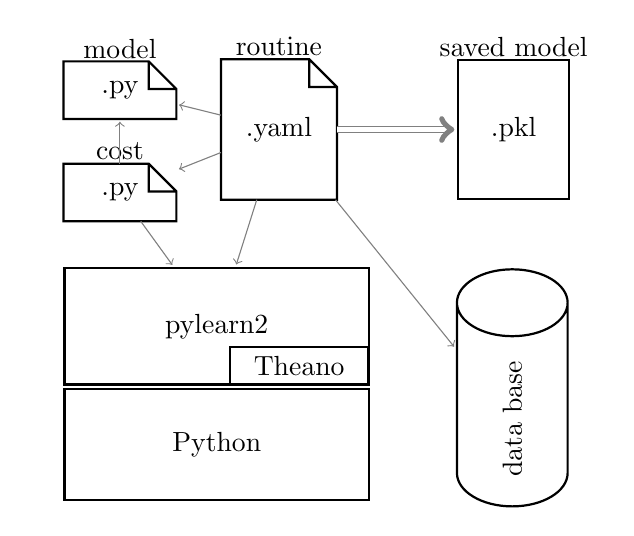
\begin{tikzpicture}[shorten >=1pt,->,draw=black!50, node distance=\layersep]
			    \tikzstyle{annot} = [text width=6em, text centered]
			    \tikzstyle{doc}  = [draw,thick,anchor=west,color=black,shape=document,minimum width=4em,minimum height=5em,inner sep=2ex]
			    \tikzstyle{doc1} = [draw,thick,anchor=west,color=black,shape=document,minimum width=4em,minimum height=2em,inner sep=1ex]
			    \tikzstyle{save} = [draw,thick,anchor=west,color=black,shape=rectangle,minimum width=4em,minimum height=5em,inner sep=1ex]
			    \tikzstyle{db}   = [draw,thick,anchor=west,color=black,cylinder,minimum width=4em,minimum height=5em,inner sep=2ex, rotate=90]
			    \tikzstyle{rect} = [draw,thick,anchor=west,color=black,shape=rectangle,minimum width=4em,minimum height=5em,]

			   	
			   	\node[doc]  (ROUT) at (2,0)   {.yaml}; \node[annot,above of=ROUT, node distance=3em] {routine};
			   	\node[doc1] (COST) at (0,-.8) {.py};   \node[annot,above of=COST, node distance=1.5em] {cost};
			   	\node[doc1] (MODL) at (0,.5)  {.py};   \node[annot,above of=MODL, node distance=1.5em] {model};
			   	\node[save] (SAVE) at (5,0)   {.pkl};  \node[annot,above of=SAVE, node distance=3em] {saved model};


			   	\node[rect, minimum width=11em, minimum height=4.2em] (PYLE)  at (0,-2.5) {pylearn2};
			   	\node[rect, minimum width=5em,  minimum height=1em]   (THEA)    at (2.1,-3) {Theano};
			   	\node[rect, minimum width=11em, minimum height=4em]   (PYTH)    at (0,-4) {Python};
			   	
			   	\node[db]   (DB)    at (5.7,-4.8) {data base};


			   	\path (ROUT) edge (PYLE);
			   	\path (ROUT) edge (COST);
			   	\path (ROUT) edge (MODL);
			   	\path (ROUT) edge (DB);
			   	\path (ROUT) edge[double distance = 1.5pt] (SAVE);
			   	\path (COST)  edge (PYLE);
			   	\path (COST)  edge (MODL);
			\end{tikzpicture}
			\caption{Graphical representation of Pylearn2's routine}
			\label{fig:pylearn2}
		\end{figure}

	\subsection{Our implementation}
		We decided to re-implement the adversarial-learning for two reasons. The first one was to get more insights on the way Pylearn2 works and the second reason was that there were no available code doing adversarial-learning. At the end, the code produced is very easy to understand. None the less, this bit of code doesn't reflect the difficulties of writing it, as there is a huge lack of documentation and proper error logs on Pylearn2.

		\vskip 1em
		We won't present here the \textbf{model} for two reasons. At first we used an implementation that provided in the library, and, secondly, because the code is hundreds of lines. How-ever, the code beneath the model does what we expected it to do. It creates a layers of Regression Logistic Units and ends up with a softmax layer.

		Then comes the implementation of the \textbf{cost}. On the constructor we define a learning epsilon value that will be able to modify when calling the routine. Then, the 'expr' function computes the adversarial-cost in a Theano-symbolic way.

		\lstset{language=Python}
		\begin{lstlisting}[basicstyle=\small,frame=single]
class AdversarialCost(DefaultDataSpecsMixin, Cost):
    # The default Cost to use with an MLP.
    supervised = True

    def __init__(self, learning_eps):
        self.learning_eps = learning_eps
        

    def expr(self, model, data, **kwargs):
    	# check input space
        space, sources = self.get_data_specs(model)
        space.validate(data)
        
        # Compute adversarial cost
        X, y = data
        alpha = .5
        adv_X = X + self.learning_eps 
        	* T.sgn(T.grad(model.cost_from_X(data),X))
        adv_data = (adv_X, y)

        return alpha*model.cost_from_X(data) 
        	+ (1-alpha)*model.cost_from_X(adv_data)

    @wraps(Cost.is_stochastic)
    def is_stochastic(self):
        return False
.
		\end{lstlisting}

		Finally, the \textbf{routine} file (the .yaml one) covers all the function calls. At first you call Pylearn2's \textit{Training} class. Then you define the model you want to train, here a ReLU shallow-neural-net. On the example below, the network is composed by 784 input units (for the MNIST database), 1200 ReLU hidden units on a single layer and a softmax output layer composed by 10 classes. Here, each of the classes will refer to a digit class. After the model comes the \textit{learning algorithm} class. We elected the Standard Gradient Descent (SDG) with some improvements: we use a batch version of it so the results comes quicker and add a momentum to the learning rate so that learning takes into consideration its previous moves when following the gradient. Still in the SDG, we elected common early-stopping stopping technique based on a validation set: we train on a testing set and, when ever the validation set show that training is over-fitting we stop the training. Furthermore, we use a rollback so that we don't consider over-fitting to early, in other words, the learning wont stop as soon as the validation states it performs worst than the train set, but we wait a hundred iteration before claiming the over-fitting (still based on the train set outperforming the validation set = over-fitting). Finally comes the cost related to the learning algorithm. Here we use the one we've shown previously: the adversarial cost. In this class comes a learning epsilon, it is the one of equation \ref{eq:sample_twist}. When given $0$, it's an usual cross-entropy learning and when given a value between $]0,1[$ it's an adversarial learning. 

		\lstset{language=Python}
		\begin{lstlisting}[basicstyle=\small,frame=single]
!obj:pylearn2.train.Train {
  dataset: &train !obj:pylearn2.datasets.
        dense_design_matrix.DenseDesignMatrix {
    X: !pkl: '/home/marc/data/mnist_train_X.pkl',
    y: !pkl: '/home/marc/data/mnist_train_y.pkl',
    y_labels: 10,
  },
  model: !obj:pylearn2.models.mlp.MLP {
    layers:[!obj:pylearn2.models.mlp.RectifiedLinear{
         layer_name: 'h0',
         dim: 1200,
         sparse_init: 15
       }, !obj:pylearn2.models.mlp.Softmax {
         layer_name: 'y',
         n_classes: 10,
         irange: 0.
       }
    ],
    nvis: 784,
  },
  algorithm: !obj:pylearn2.training_algorithms.sgd.SGD {
    batch_size: 200,
    learning_rate: .01,
    learning_rule: !obj:pylearn2.training_algorithms
        .learning_rule.Momentum {
      init_momentum: .5 },
    monitoring_dataset: {
      'train' : *train,
      'valid' : !obj:pylearn2.(...).DenseDesignMatrix {
        X: !pkl: '/home/marc/data/mnist_valid_X.pkl',
        y: !pkl: '/home/marc/data/mnist_valid_y.pkl',
        y_labels: 10,
      },
      'test' : !obj:pylearn2.(...).DenseDesignMatrix {
        X: !pkl: '/home/marc/data/mnist_test_X.pkl',
        y: !pkl: '/home/marc/data/mnist_test_y.pkl',
        y_labels: 10,
      }, },
    termination_criterion:!obj:pylearn2.
    	termination_criteria.And { criteria: [
        !obj:pylearn2.termination_criteria.MonitorBased {
            channel_name: "valid_y_misclass",
            prop_decrease: 0.,
            N: 100
        },
        !obj:pylearn2.termination_criteria.EpochCounter {
            max_epochs: 1500
        }
      ]
    },
    cost: !obj:costAdv.AdversarialCost {
      learning_eps: %(learning_eps)f }
  },
  extensions: [
    !obj:pylearn2.(...).MonitorBasedSaveBest {
       channel_name: 'valid_y_misclass',
       save_path: "%(path)s/mlp_1_%(learning_eps)s.pkl",
    }, !obj:pylearn2.(...).MomentumAdjustor {
      start: 1,
      saturate: 10,
      final_momentum: .99
    }
  ]
}
		\end{lstlisting}

		As a note, one may wonder why is the cost inside the learning algorithm. The reason is that some neural-networks can be unsupervised, meaning that their cost doesn't depends on their inputs. As a result, the learning algorithm just doesn't ask for a cost. 



\begin{appendices}
	\section{Two neurons neural network's cost}
	\label{sec:2N_NN_cost}
		Here we want to derive the cost $C$ of neural network\ref{fig:2N_NN} with respect to $x$. We first detail all the variables and then proceed to derivation.
		\begin{itemize}
			\item $C$ is the cost defined for sample $i$ as $C_i = y_i \ln(p_i) + (1-y_i)\ln(1-p_i)$, and the total cost $C$ is the mean of over the samples' costs.
			\item $p_i$ is the prediction for sample $i$. It's defined by $p_i = \sigma(z)$
			\item $\sigma(z)$ is the sigmoid function: $\sigma(z) = \frac{1}{1 + e^{-z}}$. It's derivative with respect to $z$ is $\sigma(z)(1-\sigma(z))$
			\item $z$ is a term introduced to narrow the notation. $z=W^Tx+b$.
			\item $W^T$ is the weight matrix such that $W^j$ is the weight vector for neuron $j$
			\item $b$ is a bias term. It can be considered as a weight to a feature always equal to one.
			\item $x_i$ is an input sample vector defined by its features.
		\end{itemize}
		Now, we use the chain rule to derive the Cost $C_i$ with respect to input $x$
		\begin{equation}
			\begin{split}
				\frac{\delta C_i}{\delta x} &= \frac{\delta C_i}{\delta p_i} \frac{\delta p_i}{\delta x} \\
				&= y_i \frac{1}{p_i} \frac{\delta p_i}{\delta x} + (1-y_i)\frac{1}{1-p_i} \frac{\delta (1-p_i)}{\delta x} \\
				&= \frac{y_i}{p_i} p_i(1-p_i)\frac{\delta z}{\delta x} + \frac{1-y_i}{1-p_i} -(p_i)(1-p_i) \frac{\delta z}{\delta x} \\
				&= \left( y_i (1-p_i) + (1-y_i) (-p_i)   \right) \frac{\delta z}{\delta x} \\
				&= W \left( y_i (1-p_i) + (1-y_i) (0-p_i)  \right)  \\
				&= W \left( y_i -p_i                       \right)
			\end{split}
		\end{equation}
\end{appendices}
		





\bibliographystyle{plain}
\bibliography{main}




\end{document}
